% Options for packages loaded elsewhere
\PassOptionsToPackage{unicode}{hyperref}
\PassOptionsToPackage{hyphens}{url}
\PassOptionsToPackage{dvipsnames,svgnames,x11names}{xcolor}
%
\documentclass[
  12pt]{article}

\usepackage{amsmath,amssymb}
\usepackage{iftex}
\ifPDFTeX
  \usepackage[T1]{fontenc}
  \usepackage[utf8]{inputenc}
  \usepackage{textcomp} % provide euro and other symbols
\else % if luatex or xetex
  \usepackage{unicode-math}
  \defaultfontfeatures{Scale=MatchLowercase}
  \defaultfontfeatures[\rmfamily]{Ligatures=TeX,Scale=1}
\fi
\usepackage{lmodern}
\ifPDFTeX\else  
    % xetex/luatex font selection
\fi
% Use upquote if available, for straight quotes in verbatim environments
\IfFileExists{upquote.sty}{\usepackage{upquote}}{}
\IfFileExists{microtype.sty}{% use microtype if available
  \usepackage[]{microtype}
  \UseMicrotypeSet[protrusion]{basicmath} % disable protrusion for tt fonts
}{}
\usepackage{xcolor}
\setlength{\emergencystretch}{3em} % prevent overfull lines
\setcounter{secnumdepth}{5}
% Make \paragraph and \subparagraph free-standing
\ifx\paragraph\undefined\else
  \let\oldparagraph\paragraph
  \renewcommand{\paragraph}[1]{\oldparagraph{#1}\mbox{}}
\fi
\ifx\subparagraph\undefined\else
  \let\oldsubparagraph\subparagraph
  \renewcommand{\subparagraph}[1]{\oldsubparagraph{#1}\mbox{}}
\fi


\providecommand{\tightlist}{%
  \setlength{\itemsep}{0pt}\setlength{\parskip}{0pt}}\usepackage{longtable,booktabs,array}
\usepackage{calc} % for calculating minipage widths
% Correct order of tables after \paragraph or \subparagraph
\usepackage{etoolbox}
\makeatletter
\patchcmd\longtable{\par}{\if@noskipsec\mbox{}\fi\par}{}{}
\makeatother
% Allow footnotes in longtable head/foot
\IfFileExists{footnotehyper.sty}{\usepackage{footnotehyper}}{\usepackage{footnote}}
\makesavenoteenv{longtable}
\usepackage{graphicx}
\makeatletter
\def\maxwidth{\ifdim\Gin@nat@width>\linewidth\linewidth\else\Gin@nat@width\fi}
\def\maxheight{\ifdim\Gin@nat@height>\textheight\textheight\else\Gin@nat@height\fi}
\makeatother
% Scale images if necessary, so that they will not overflow the page
% margins by default, and it is still possible to overwrite the defaults
% using explicit options in \includegraphics[width, height, ...]{}
\setkeys{Gin}{width=\maxwidth,height=\maxheight,keepaspectratio}
% Set default figure placement to htbp
\makeatletter
\def\fps@figure{htbp}
\makeatother

\addtolength{\oddsidemargin}{-.5in}%
\addtolength{\evensidemargin}{-1in}%
\addtolength{\textwidth}{1in}%
\addtolength{\textheight}{1.7in}%
\addtolength{\topmargin}{-1in}%
\makeatletter
\@ifpackageloaded{caption}{}{\usepackage{caption}}
\AtBeginDocument{%
\ifdefined\contentsname
  \renewcommand*\contentsname{Table of contents}
\else
  \newcommand\contentsname{Table of contents}
\fi
\ifdefined\listfigurename
  \renewcommand*\listfigurename{List of Figures}
\else
  \newcommand\listfigurename{List of Figures}
\fi
\ifdefined\listtablename
  \renewcommand*\listtablename{List of Tables}
\else
  \newcommand\listtablename{List of Tables}
\fi
\ifdefined\figurename
  \renewcommand*\figurename{Figure}
\else
  \newcommand\figurename{Figure}
\fi
\ifdefined\tablename
  \renewcommand*\tablename{Table}
\else
  \newcommand\tablename{Table}
\fi
}
\@ifpackageloaded{float}{}{\usepackage{float}}
\floatstyle{ruled}
\@ifundefined{c@chapter}{\newfloat{codelisting}{h}{lop}}{\newfloat{codelisting}{h}{lop}[chapter]}
\floatname{codelisting}{Listing}
\newcommand*\listoflistings{\listof{codelisting}{List of Listings}}
\makeatother
\makeatletter
\makeatother
\makeatletter
\@ifpackageloaded{caption}{}{\usepackage{caption}}
\@ifpackageloaded{subcaption}{}{\usepackage{subcaption}}
\makeatother
\ifLuaTeX
  \usepackage{selnolig}  % disable illegal ligatures
\fi
\usepackage[]{natbib}
\bibliographystyle{agsm}
\usepackage{bookmark}

\IfFileExists{xurl.sty}{\usepackage{xurl}}{} % add URL line breaks if available
\urlstyle{same} % disable monospaced font for URLs
\hypersetup{
  pdftitle={Integrated Likelihood Inference in Poisson Distributions},
  pdfauthor={Timothy Ruel},
  pdfkeywords={Directly standardized rate, Integrated likelihood ratio
statistic, Maximum integrated likelihood estimator, Profile
likelihood, Weighted sum, Zero score expectation parameter},
  colorlinks=true,
  linkcolor={blue},
  filecolor={Maroon},
  citecolor={Blue},
  urlcolor={Blue},
  pdfcreator={LaTeX via pandoc}}


\begin{document}


\def\spacingset#1{\renewcommand{\baselinestretch}%
{#1}\small\normalsize} \spacingset{1}


%%%%%%%%%%%%%%%%%%%%%%%%%%%%%%%%%%%%%%%%%%%%%%%%%%%%%%%%%%%%%%%%%%%%%%%%%%%%%%

\title{\bf Integrated Likelihood Inference in Poisson Distributions}
\author{
Timothy Ruel\\
Department of Statistics and Data Science, Northwestern University\\
}
\maketitle

\bigskip
\bigskip
\begin{abstract}
The text of your abstract. 200 or fewer words.
\end{abstract}

\noindent%
{\it Keywords:} Directly standardized rate, Integrated likelihood ratio
statistic, Maximum integrated likelihood estimator, Profile
likelihood, Weighted sum, Zero score expectation parameter
\vfill

\newpage
\spacingset{1.9} % DON'T change the spacing!

\section{Introduction}\label{sec-intro}

Consider a vector \(\theta = (\theta_1, ..., \theta_n)\) in which each
component represents the mean of a distinct Poisson process. The purpose
of this paper is to discuss the task of conducting likelihood-based
inference for a real-valued parameter of interest
\(\psi = \tau(\theta)\). In particular, we will examine the utility of
the integrated likelihood function as a tool for obtaining interval and
point estimates for \(\psi\), using the performance of the more easily
calculated profile likelihood as a benchmark.

We may obtain a sample of values from each Poisson process through
repeated measurements of the number of events it generates over a fixed
period of time. Suppose we have done so, and let \(X_{ij}\) represent
the \(j\)th count from the \(i\)th sample, so that
\(X_{ij} \sim \text{Poisson}(\theta_i)\) for \(i = 1, ..., n\) and
\(j = 1, ..., m_i.\) The probability mass function (pmf) for a single
observation \(X_{ij} = x_{ij}\) is
\begin{equation}\phantomsection\label{eq-1}{
p(x_{ij}; \> \theta_i) = \frac{e^{-\theta_i} \theta_i ^ {x_{ij}}}{x_{ij}!}, \> \> x_{ij} = 0, 1, 2, ... ; \> \> \theta_i > 0.
}\end{equation}

Denote the sample of counts from the \(i\)th process by the vector
\(X_{i\bullet} = (X_{i1}, ..., X_{im_i})\), its associated mean by
\(\bar{X}_{i \bullet} = \frac{1}{m_i} \sum_{j = 1}^{m_i} X_{ij}\), and
assume that all of the counts both within and between samples are
measured independently. The likelihood function for an individual
component \(\theta_i\) based on the data \(X_{i\bullet} = x_{i\bullet}\)
is then equal to the product of the individual probabilities of the
observed counts, i.e. \begin{equation}\phantomsection\label{eq-2}{
\begin{aligned}
L(\theta_i; x_{i\bullet}) &= \prod_{j=1}^{m_i} p(x_{ij}; \theta_i) \\
                          &= \prod_{j=1}^{m_i} \frac{e^{-\theta_i} \theta_i ^ {x_{ij}}}{x_{ij}!} \\
                          &= \Bigg(\prod_{j=1}^{m_i} e^{-\theta_i}\Bigg) \Bigg(\prod_{j=1}^{m_i}\theta_i^{x_{ij}}\Bigg) \Bigg(\prod_{j=1}^{m_i} x_{ij}!\Bigg)^{-1} \\
                          &= \bigg(e^{-\sum_{j=1}^{m_i}\theta_i}\bigg) \bigg(\theta_i^{\sum_{j=1}^{m_i}x_{ij}}\bigg) \Bigg(\prod_{j=1}^{m_i} x_{ij}!\Bigg)^{-1} \\
                          &= e^{-m_i\theta_i}\theta_i^{m_i\bar{x}_{i\bullet}}\Bigg(\prod_{j=1}^{m_i} x_{ij}!\Bigg)^{-1}.
\end{aligned}
}\end{equation}

Since \(L\) is only useful to the extent that it informs our
understanding of the value of \(\theta_i\), we are free to replace it
with any other function differing from it by just a (nonzero)
multiplicative term that is constant with respect to \(\theta_i\),
provided that the result still satisfies the necessary regularity
conditions, as this will not change any conclusions regarding
\(\theta_i\) that we draw from it. Hence, we may safely discard the term
in parentheses on the final line of Equation~\ref{eq-2} as it does not
depend on \(\theta_i\) and instead simply write
\begin{equation}\phantomsection\label{eq-3}{
L(\theta_i; x_{i\bullet}) = e^{-m_i\theta_i}\theta_i^{m_i\bar{x}_{i\bullet}}.
}\end{equation}

It will generally be more convenient to work with the log-likelihood
function, which is given by \begin{equation}\phantomsection\label{eq-4}{
\begin{aligned}
\ell(\theta_i; x_{i\bullet}) &= \log L(\theta_i; x_{i\bullet}) \\
                           &= \log \Big(e^{-m_i\theta_i}\theta_i^{m_i\bar{x}_{i\bullet}}\Big) \\
                           &= -m_i\theta_i + m_i \bar{x}_{i\bullet} \log \theta_i \\
                           &=  m_i\big(\bar{x}_{i\bullet} \log\theta_i - \theta_i \big).
\end{aligned}
}\end{equation} The sum of the log-likelihood functions for each
component of \(\theta\) then forms the basis of the log-likelihood
function for \(\theta\) itself:
\begin{equation}\phantomsection\label{eq-5}{
\begin{aligned}
\ell(\theta; x_{1\bullet}, ..., x_{n\bullet}) &= \log L(\theta; x_{1\bullet}, ..., x_{n\bullet}) \\
                                              &= \log \Bigg(\prod_{i=1}^n L(\theta_i; x_{i\bullet})\Bigg) \\
                                              &= \sum_{i=1}^n \log L(\theta_i; x_{i\bullet}) \\
                                              &= \sum_{i=1}^n \ell(\theta_i; x_{i\bullet}) \\
                                              &= \sum_{i=1}^n m_i\big(\bar{x}_{i\bullet} \log\theta_i - \theta_i \big).
\end{aligned}
}\end{equation}

We can derive the maximum likelihood estimate (MLE) for \(\theta_i\) by
differentiating Equation~\ref{eq-4} with respect to \(\theta_i\),
setting the result equal to 0, and solving for \(\theta_i\). This gives
the nice result that the MLE is simply equal to the mean of the sample
of data \(X_{i\bullet}\). That is,
\begin{equation}\phantomsection\label{eq-6}{
\hat{\theta}_i = \bar{X}_{i\bullet}.
}\end{equation} Similarly, the MLE for the full parameter \(\theta\) is
just the vector of MLEs for its individual components:
\begin{equation}\phantomsection\label{eq-7}{
\hat{\theta} \equiv (\hat{\theta}_1, ..., \hat{\theta}_n) = (\bar{X}_{1\bullet}, ..., \bar{X}_{n\bullet}).
}\end{equation}

\section{Pseudolikelihoods}\label{pseudolikelihoods}

Let \(\Theta \subseteq \mathbb{R}^n_+\) represent the space of possible
values for \(\theta\) and suppose we have a real-valued \emph{parameter
of interest} \(\psi = \tau(\theta)\), where \(\tau: \Theta \to \Psi\) is
a known function with at least two continuous derivatives. Though it is
not strictly necessary, in order to align with the tendency of
researchers to focus on one-dimensional summaries of vector quantities
we will assume for our purposes that \(\psi\) is a scalar,
i.e.~\(\Psi \subseteq \mathbb{R}\).

This reduced dimension of \(\Psi\) relative to \(\Theta\) implies the
existence of a \emph{nuisance parameter}
\(\lambda \in \Lambda \subseteq \mathbb{R}^{n-1}\). As its name
suggests, \(\lambda\) tends to obfuscate or outright preclude inference
regarding \(\psi\) and typically must be eliminated from the likelihood
before proceeding. The product of this elimination is called a
\emph{pseudolikelihood function}. Any function of the data and \(\psi\)
alone could theoretically be considered a pseudolikelihood, though
course in practice some are more useful than others.

If we let
\(\Theta_{\psi} = \{\theta \in \Theta: \> \tau(\theta) = \psi \},\) then
associated with each \(\psi \in \Psi\) is the set of likelihood values
\(\mathcal{L}_{\psi} = \{L(\theta): \> \theta \in \Theta_{\psi}\}.\) For
a given value of \(\psi\), there may exist multiple corresponding values
of \(\lambda\).

We can construct pseudolikelihoods for \(\psi\) through clever choices
by which to summarize \(\mathcal{L}_{\psi}\) over all possible values of
\(\lambda\). Among the most popular methods of summary are profiling
(i.e.~maximization), conditioning, and integration, each with respect to
the nuisance parameter. These summaries do come at a cost, however;
eliminating a model's nuisance parameter from its likelihood almost
always sacrifices some information about its parameter of interest as
well. One measure of a good pseudolikelihood, therefore, is the balance
it strikes between the amount of information it retains about \(\psi\)
and the ease with which it can be computed.

\subsection{The Profile Likelihood}\label{the-profile-likelihood}

The most straightforward method we can use to construct a
pseudolikelihood (or equivalently, a pseudo-log-likelihood) function for
\(\psi\) is usually to find the maximum of \(\ell(\theta)\) over all
possible of values of \(\theta\) for each value of \(\psi\). This yields
what is known as the \emph{profile} log-likelihood function, formally
defined as \begin{equation}\phantomsection\label{eq-8}{
\ell_p(\psi) = \sup_{\theta \in \Theta: \> \tau(\theta) = \psi} \ell(\theta), \> \> \psi \in \Psi.
}\end{equation} In the case where an explicit nuisance parameter
\(\lambda\) exists so that \(\theta\) may be written as
\(\theta = (\psi, \lambda)\), Equation~\ref{eq-8} is equivalent to
replacing \(\lambda\) with \(\hat{\lambda}_{\psi}\), its conditional MLE
given \(\psi\): \begin{equation}\phantomsection\label{eq-9}{
\ell_p(\psi) = \ell(\psi, \hat{\lambda}_{\psi}).
}\end{equation}

Historically, the efficiency with which the profile is capable of
producing accurate estimates of \(\psi\) relative to its ease of
computation has made it the method of choice for statisticians when
performing likelihood-based inference regarding a parameter of interest.
Examples of profile-based statistics are the MLE for \(\psi\), i.e.,
\begin{equation}\phantomsection\label{eq-10}{
\hat{\psi} = \underset{\psi \in \Psi}{\arg\sup} \> \ell_p(\psi),
}\end{equation} and the signed likelihood ratio statistic for \(\psi\),
given by \begin{equation}\phantomsection\label{eq-10}{
R_{\psi} = \text{sgn}(\hat{\psi} - \psi)(2(\ell_p(\hat{\psi}) - \ell_p(\psi)))^{\frac{1}{2}}.
}\end{equation}

\subsection{The Integrated Likelihood}\label{the-integrated-likelihood}

The \emph{integrated likelihood} for \(\psi\) seeks to summarize
\(\mathcal{L}_{\psi}\) by its average value with respect to some weight
function \(\pi\) over the space \(\Theta_{\psi}\). From a theoretical
standpoint, this is preferable to the maximization procedure found in
the profile likelihood as it naturally incorporates our uncertainty
regarding the nuisance parameter's true value into the resulting
pseudolikelihood. The general form of an integrated likelihood function
is given \begin{equation}\phantomsection\label{eq-11}{
\bar{L}(\psi) = \int_{\Theta_{\psi}}L(\theta)\pi(\theta; \psi)d\theta.
}\end{equation}

It is up to the researcher to choose the weight function
\(\pi(\cdot; \psi)\), which plays an important role in the properties of
the resulting integrated likelihood. Severini (2007) developed a method
for re-parameterizing \(\lambda\) that makes the integrated likelihood
relatively insensitive to the exact weight function chosen. Using this
new parameterization, we have great flexibility in choosing our weight
function; as long as it does not depend on the parameter of interest,
the integrated likelihood that is produced will enjoy many desirable
frequency properties.

\section{Application to Poisson
Models}\label{application-to-poisson-models}

We now turn our attention to the task of using the ZSE parameterization
to construct an integrated likelihood that can be used to make
inferences regarding a parameter of interest derived from the Poisson
model described in the introduction. We will

\section{Estimating the Weighted Sum of Poisson
Means}\label{estimating-the-weighted-sum-of-poisson-means}

Consider the weighted sum \[Y = \sum_{i=1}^n w_iX_i,\] where each
\(w_i\) is a known constant greater than zero. Suppose we take for our
parameter of interest the expected value of this weighted sum, so that
\[\psi \equiv \text{E}(Y) = \sum_{i=1}^n w_i\theta_i.\]

\subsection{Examples}\label{examples}

\section{Zero-Inflated Poisson
Regression}\label{zero-inflated-poisson-regression}

A sample of count data is called \emph{zero-inflated} when it contains
an excess amount of zero-valued observations. A common tactic to account
for this excess is to model the data using a mixture of two processes,
one that generates zeros and another that generates counts, some of
which may also be zeros. When this count-generating process follows a
Poisson distribution, we call the resulting mixture a zero-inflated
Poisson (ZIP) model.

Let \(U \sim \text{Bernoulli}(1 - \pi)\) and
\(V \sim \text{Poisson}(\mu)\) Suppose \(U\) and \(V\) are independent
and let \(W = UV\). Then \(W \sim \text{ZIP}(\mu, \pi)\). Note that
\(W = 0\) when either \(U = 0\) or \(V = 0\) so that \[
\begin{aligned}
\mathbb{P}(W = 0) &= \mathbb{P}(U = 0 \cup V = 0) \\
                  &= \mathbb{P}(U = 0) + \mathbb{P}(V = 0) - \mathbb{P}(U = 0 \cap V = 0) \\
                  &= \mathbb{P}(U = 0) + \mathbb{P}(V = 0) - \mathbb{P}(U = 0)\mathbb{P}(V = 0) \\
                  &= \pi + e^{-\mu} - \pi e^{-\mu} \\ 
                  &= \pi + (1 - \pi)e^{-\mu}.
\end{aligned}
\] In order for \(W\) to take on a value \(w > 0\), we must have
\(U = 1\) and \(V = w\). That is, \[
\begin{aligned}
\mathbb{P}(W = w) &= \mathbb{P}(U = 1 \cap V = w) \\
                  &= \mathbb{P}(U = 1)\mathbb{P}(V = w) \\
                  &= (1-\pi)\frac{e^{-\mu}\mu^w}{w!}, \> \> w = 1, 2, ...
\end{aligned}
\] Thus, the full probability mass function for a ZIP random variable is
given by \[
\mathbb{P}(W = w) = \begin{cases}
               \pi + (1 - \pi)e^{-\mu}, &w =0 \\
               (1-\pi)\frac{e^{-\mu}\mu^w}{w!}, & w = 1, 2, ...
            \end{cases}
\]

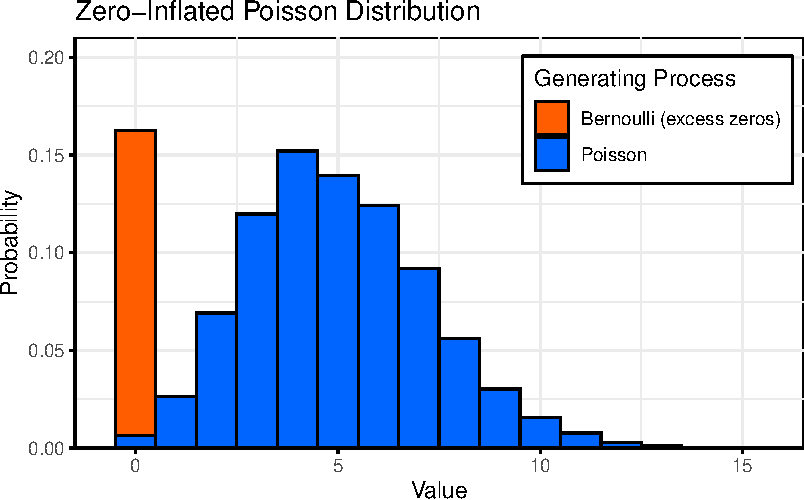
\includegraphics{Paper_files/figure-pdf/unnamed-chunk-1-1.pdf}


  \bibliography{bibliography.bib}


\end{document}
